\documentclass[a4paper,pra,aps,twocolumn,superscriptaddress,10pt,final]{revtex4-2}
\usepackage[pretty,uselistings]{revquantum}
% \usepackage[brazil]{babel}
\usepackage[T1]{fontenc}
\usepackage[utf8]{inputenc}
\usepackage{stmaryrd} 
\SetSymbolFont{stmry}{bold}{U}{stmry}{m}{n} 
\usepackage{bm}
\usepackage{amsmath}
\usepackage{amssymb}
\usepackage{amsfonts}
\usepackage{silence}
\WarningFilter{revtex4-2}{Repair the float}
\usepackage{anyfontsize}
\usepackage{lipsum}
\usepackage{float}
\usepackage{graphicx}
\usepackage{multirow}
% \usepackage{multicol}
\usepackage{wrapfig}
\usepackage[paperwidth=210mm,paperheight=297mm,centering,hmargin=2cm,vmargin=2.5cm]{geometry}
% \usepackage{physics}
\usepackage{siunitx}
\usepackage{tabularray}
\UseTblrLibrary{booktabs}
%=============================================================================
% FRONT MATTER
%=============================================================================
% \graphicspath{{..imgs/}}

\begin{document}

\title{Atividade prática da disciplina de Circuitos Elétricos 1}

\author{Paulo Vinicius Pereira Pinheiro}
\email{paulovpp@gmail.com}
\affiliation{UNINTER - Centro Universitário Internacional}
\affiliation{RU: 3760288}
\affiliation{PAP: Juazeiro do Norte, CE. CEP: 63.000-000}

\date{\today}

\begin{abstract}
    A crescente necessidade por segurança nas transações online traz à tona um problema de grande complexidade: até quando os protocolos atuais de segurança da informação serão capazes de nos manter seguros? Inúmeros são casos de quebra de segurança ou vazamento de dados. Mesmo com uma grande quantidade de métodos utilizados para comunicação segura, não há garantias de plena segurança para nenhum deles. Dentre todos os métodos existentes, destaca-se a criptografia. De forma simétrica ou assimétrica, o ato de criptografar uma mensagem é torná-la inelegível a aqueles à quem a mensagem não se destina. A criptografia é um dos tópicos abordados na disciplina de matemática computacional do curso de engenharia da computação da UNINTER. E o trabalho realizado trata do assunto de forma aplicada. Através da Cifra de Feistel, pode-se compreender com mais clareza os procedimentos de codificação e decodificação de mensagens criptografados. Pra tal, são solicitados os seguintes procedimentos: que sejam codificados os 4 primeiros caracteres do primeiro nome do aluno utilizando-se a cifra simétrica de Feistel com apenas 2 estágios, utilizando o último dígito do RU não nulo, $K$,  como a chave criptográfica para ambos os estágios. Deve-se utilizar também como função $F$ um shift left, cíclico, de $K$ posições. Solicita-se também que a mensagem codificada seja preparada para transmissão e que, em seguida, haja o processo de decodificação, comprovando assim a reciprocidade do processo.
    
    
\end{abstract}

\maketitle

%=============================================================================
% MAIN DOCUMENT
%=============================================================================

\section{Introdução}
\label{sec:intro}

    Criptografia é o processo de codificar ou embaralhar uma mensagem que se deseja transmitir, de tal modo que apenas aquele à quem a mensagem se destine tenha meios para identificar seu conteúdo. Inúmeros são os usos da criptografia para comunicação segura, como em transações financeiras, governamentais e empresariais. 

\section{Procedimento experimental}
\label{sec:proced_exp}

    A presente seção tem por objetivo apresentar a metodologia para os procedimentos realizados na atividade em questão. Destaca-se que como a atividade é bastante extensa, esta seção e as subsequentes foram subdivididas em quatro partes, correspondendo cada uma a uma questão prática proposta.

    Todos os experimentos em resumo solicitam sua montagem real em placa de teste, a respectiva medição dos valores de tensão e corrente para diversos parâmetros e a comparação com a simulação realizada por software competente. Os dados obtidos e sua análise são apresentados na seção seguinte~\ref{sec:analise_resultados}.

\subsection{Experimento 1: Lei de Ohm}
\label{subsec:exp_lei_ohm}

    Neste primeiro experimento, foi solicitada a montagem real do circuito apresentado na Figura~\ref{fig:circuito1} e sua simulação utilizando um circuito digital. O circuito é composto apenas pela fonte de tensão contínua e um resistor com o valor deduzido do RU do aluno. No caso do autor deste trabalho, com o RU de número 3760288, o valor do resistor é de $\qty{880}{\ohm}$. Como não há um resistor deste valor, foram utilizados dois resistores em uma associação em série, com os valores iguais a $\qty{560}{\ohm}$ e $\qty{330}{\ohm}$, o que resulta na resistência equivalente igual a $\qty{890}{\ohm}$

    \begin{figure}[H]
        \centering
        \caption{Circuito elétrico do Experimento 1}
        \includegraphics[width=0.4\textwidth]{imgs/fig1.png}\\
        \scriptsize{Fonte: Elaboração própria.}
        \label{fig:circuito1}
    \end{figure}

    A confecção do circuito em placa de testes \emph{protoboard} está apresentada na figura \ref{fig:protoboard1}. 
    
    \begin{figure}[H]
        \centering
        \caption{Circuito elétrico do experimento 1 em montagem real.}
        \includegraphics[width=0.4\textwidth]{imgs/fig3.png}\\
        \scriptsize{Fonte: Elaboração própria.}
        \label{fig:protoboard1}
    \end{figure}

    Da mesma forma, também foi solicitada a simulação do circuito em um computador. A simulação foi realizada utilizando a plataforma \emph{MultiSim} e o circuito simulado está apresentado na figura \ref{fig:circuito1}.

\subsection{Experimento 2: Divisor de tensão}
\label{subsec:exp_div_tens}

    Neste experimento, foi solicitada a montagem real do circuito apresentado na figura~\ref{fig:circuito2} e sua simulação utilizando um circuito digital. Trata-se de um  circuito  com uma associação em série de resistores. Foram utilizados três resistores com valores previamente definidos, em uma associação em série, com os valores iguais a $\qty{560}{\ohm}$, $\qty{1}{\kilo\ohm}$ e $\qty{2,2}{\kilo\ohm}$, o que resulta na resistência equivalente igual a $\qty{1}{\kilo\ohm}$. Os valores de tensão fornecidos variam entre 5, 7, 10 e 12$\unit{\volt}$.
    
    \begin{figure}[H]
        \centering
        \caption{Circuito elétrico do Experimento 2}
        \includegraphics[width=0.4\textwidth]{imgs/circuito2.png}\\
        \scriptsize{Fonte: Elaboração própria.}
        \label{fig:circuito2}
    \end{figure}
    
    A confecção do circuito em placa de testes \emph{protoboard} está apresentada na figura \ref{fig:protoboard2}. 
    
    \begin{figure}[htpb]
        \centering
        \caption{Circuito elétrico do Experimento 2 - montagem real.}
        \includegraphics[width=0.4\textwidth]{imgs/protoboard2.png}\\
        \scriptsize{Fonte: Elaboração própria.}
        \label{fig:protoboard2}
    \end{figure}
    
    Da mesma forma, também foi solicitada a simulação do circuito em um computador. A simulação foi realizada utilizando a plataforma \emph{MultiSim} e o circuito simulado está apresentado na figura \ref{fig:circuito2}.


\subsection{Experimento 3: Divisor de corrente}
\label{subsec:exp_div_corr}


    Para o experimento 3, um divisor de corrente foi solicitado. Os valores das resistências são idênticas ao experimento da subseção anterior (\ref{subsec:exp_div_tens}). A representação do circuito está apresentada na Figura~\ref{fig:circuito3}. Novamente os valores de tensão devem variar entre 5, 7, 10 e 12$\unit{\volt}$.

    \begin{figure}[H]
        \centering
        \caption{Circuito elétrico do Experimento 3}
        \includegraphics[width=0.4\textwidth]{imgs/circuito3.png}\\
        \scriptsize{Fonte: Elaboração própria.}
        \label{fig:circuito3}
    \end{figure}

    A montagem experimental é mostrada na Figura~\ref{fig:protoboard3}.

    \begin{figure}[H]
        \centering
        \caption{Circuito elétrico do Experimento 3 - montagem real.}
        \includegraphics[width=0.4\textwidth]{imgs/protoboard3.png}\\
        \scriptsize{Fonte: Elaboração própria.}
        \label{fig:protoboard3}
    \end{figure}

\subsection{Experimento 4: Equivalente de Thevenin}
\label{subsec:exp_equiv_the}

    Um experimento para o equivalente de Thevenin foi solicitado. O circuito apresentado na Figura~\ref{fig:circuito4} é composto por duas fontes de tensão contínua e alguns resistores de valores pré-definidos.

    \begin{figure}[H]
        \centering
        \caption{Circuito elétrico do Experimento 4.}
        \includegraphics[width=0.4\textwidth]{imgs/circuito4.png}\\
        \scriptsize{Fonte: Elaboração própria.}
        \label{fig:circuito4}
    \end{figure}

    A confecção do circuito em placa de testes \emph{protoboard} está apresentada na figura \ref{fig:protoboard4}.

    \begin{figure}[H]
        \centering
        \caption{Circuito elétrico do Experimento 4 - montagem real.}
        \includegraphics[width=0.4\textwidth]{imgs/protoboard4.png}\\
        \scriptsize{Fonte: Elaboração própria.}
        \label{fig:protoboard4}
    \end{figure}
%----------------------------------------------------------------------------------------------------------

\section{Análise e Resultados}
\label{sec:analise_resultados}

    Nesta seção serão apresentados os dados coletados das montagens reais dos experimentos, bem como serão realizadas as comparações com os valores obtidos das simulações computacionais e suas devidas elucidações.
    
\subsection{Experimento 1: Lei de Ohm}
\label{subsec:ana_exp1}

    A partir da montagem real do experimento sobre a lei de Ohm (apresentado na Figura~\ref{fig:protoboard1}) e sua simulação computacional (Figura~\ref{fig:circuito1}), juntamente com os cálculos teóricos foi criada a Tabela~\ref{tab:table_exp1_data} com os valores coletados. Mais uma imagem referente a simulação também é apresentada na Figura~\ref{fig:simula01}, essa com a prévia dos dados medidos para o valor de tensão $\qty{5,02}{\volt}$. Tal valor de tensão foi utilizado para que a simulação ofereça mais precisão com os dados coletados. Os valores de corrente medidos no circuito experimental também estão inseridos na tabela.

    \begin{table}[H]
        \caption{Valores obtidos para o experimento 1.}
        \label{tab:table_exp1_data}
        \begin{tabular}{cccccc}
            \hline
            \multirow{2}{*}{\textbf{V (V)}} &
            \multirow{2}{*}{\textbf{\begin{tabular}[c]{@{}c@{}}R\\ (ohms)\end{tabular}}} &
            \multicolumn{3}{c}{\textbf{Corrente (mA)}} &
            \multirow{2}{*}{\textbf{\begin{tabular}[c]{@{}c@{}}Erro\\ Experim.\end{tabular}}} \\ \cline{3-5}
            &     & \multicolumn{1}{c}{\textbf{Teórica}} & \multicolumn{1}{c}{\textbf{Simulada}} & \textbf{Experim.} &         \\ \hline
            0  & 890 & \multicolumn{1}{c}{0}                & \multicolumn{1}{c}{0}                 & 0                     & 0\%     \\ \hline
            5  & 890 & \multicolumn{1}{c}{5,65}             & \multicolumn{1}{c}{5,64}              & 5,38                  & 4,78\%  \\ \hline
            7  & 890 & \multicolumn{1}{c}{7,86}             & \multicolumn{1}{c}{7,83}              & 7,04                  & 10,43\% \\ \hline
            10 & 890 & \multicolumn{1}{c}{11,24}            & \multicolumn{1}{c}{11,33}             & 10,78                 & 4,09\%  \\ \hline
            12 & 890 & \multicolumn{1}{c}{13,31}            & \multicolumn{1}{c}{13,32}             & 12,82                 & 3,68\%  \\ \hline
        \end{tabular}
    \end{table}

    Para a simulação computacional, a Figura \ref{fig:simula01} apresenta na própria simulação um exemplo dos resultados obtidos para o valor de tensão $\qty{5,02}{\volt}$. O restante dos valores de tensão usados não é mostrado.

    \begin{figure}[H]
        \centering
        \caption{Simulação computacional do Experimento 1 - Lei de ohm.}
        \includegraphics[width=0.4\textwidth]{imgs/Ana01.png}\\
        \scriptsize{Fonte: Elaboração própria.}
        \label{fig:simula01}
    \end{figure}

    Também é solicitado o cálculo do erro experimental, mostrado na última coluna da tabela~\ref{tab:table_exp1_data}. A razão por trás dos erros pode ser encontrada nas condições experimentais de montagem, temperatura e o erro inerente dos componentes. Os resistores utilizados possuem tolerância de até 10\%. Há também o fato dos terminais dos mesmos serem de espessura muito menor que o orifício da placa de testes, causando possíveis erros de contato. A fonte de tensão utilizada não possui ajuste com sensibilidade suficiente e, junto com o erro inerente às medições, dos multímetros, constituem a origem da maior parte dos erros mostrados.

    Solicita-se também uma curva de corrente x tensão, com sua curva de tendência, para verificação visual do erro previamente mostrado. A Figura~\ref{fig:curva_exp1} mostra a curva:

    \begin{figure}[H]
        \centering
        \caption{Curva de corrente x tensão do Experimento 1.}
        \includegraphics[width=0.4\textwidth]{imgs/graph_exp1_1.png}\\
        % \scriptsize{Fonte: Elaboração própria.}
        \label{fig:curva_exp1}
    \end{figure}

    Com os valores de tensão e corrente obtidos, é possível calcular os valores de potência dissipada pelos resistores. Na Tabela~\ref{tab:table_exp1_pot} estão apresentados os valores e o erro experimental obtido.         

    \begin{table}[H]
        \caption{Dados do problema.}
        \label{tab:table_exp1_pot}
        \begin{tabular}{cccccc}
            \hline
            \multirow{2}{*}{\textbf{V (V)}} &
            \multirow{2}{*}{\textbf{\begin{tabular}[c]{@{}c@{}}R\\ (ohms)\end{tabular}}} &
            \multicolumn{3}{c}{\textbf{Potencia (W)}} &
            \multirow{2}{*}{\textbf{\begin{tabular}[c]{@{}c@{}}Erro\\ Experim.(\%)\end{tabular}}} \\ \cline{3-5}
            &
            &
            \multicolumn{1}{c}{\textbf{\begin{tabular}[c]{@{}c@{}}Teórica\end{tabular}}} &
            \multicolumn{1}{c}{\textbf{\begin{tabular}[c]{@{}c@{}}Simulada\end{tabular}}} &
            \textbf{\begin{tabular}[c]{@{}c@{}}Experim.\end{tabular}} &
            \\ \hline
            0  & 890 & \multicolumn{1}{c}{0}      & \multicolumn{1}{c}{0}      & 0      & 0,00\%  \\ \hline
            5  & 890 & \multicolumn{1}{c}{28,25}  & \multicolumn{1}{c}{28,2}   & 26,9   & 4,78\%  \\ \hline
            7  & 890 & \multicolumn{1}{c}{55,02}  & \multicolumn{1}{c}{54,81}  & 49,28  & 10,43\% \\ \hline
            10 & 890 & \multicolumn{1}{c}{112,4}  & \multicolumn{1}{c}{113,3}  & 107,8  & 4,09\%  \\ \hline
            12 & 890 & \multicolumn{1}{c}{159,72} & \multicolumn{1}{c}{159,84} & 153,84 & 3,68\%  \\ \hline
        \end{tabular}
    \end{table}

    Novamente percebe-se taxas de erro consideráveis. Da mesma forma como elucidado anteriormente, as taxas de erro estão embasadas em fatores como temperatura, tolerância dos componentes e possíveis erros de contato na montagem experimental. Cita-se também possíveis erros nos valores de tensão fornecidos pela fonte simétrica, como também nos equipamentos de medida utilizados.

\subsection{Experimento 2: Divisor de tensão}
\label{subsec:ana_div_tens}



\subsection{Experimento 3: Divisor de corrente}
\label{subsec:ana_div_corr}


\subsection{Experimento 4: Equivalente de Thevenin}
\label{subsec:ana_equiv_the}


\section{Conclusão}
\label{sec:conclusion}
    
    Neste trabalho foram realizadas a codificação e decodificação de uma mensagem pela Cifra de Feister, um modelo de criptografia de chave simétrica e de bloco geralmente utilizada com 64 bits. A mensagem original foi determinada a partir dos primeiros quatro caracteres do primeiro nome do autor. A função $F$ solicitada como foi a \textit{shift left} cíclico pelo número de vezes correspondente ao último dígito não inteiro do RU. E o número de interações solicitado para cada processo foi de duas iterações com a mesma chave cada.
    
    A seção de desenvolvimento foi dividida em duas partes, para os processos de codificação e decodificação correspondentemente. Tabelas foram apresentadas com o passos intermediários e os resultados preliminares das operações. As mensagens codificada e decodificada podem ser encontradas correspondentemente nas tabelas Os resultados estão de acordo com o solicitado no enunciado do trabalho.

    Conclui-se também que a Cifra de César possui um baixo custo de processamento para codificação e decodificação, já que é realizada em bloco. Porém, como trata-se de uma cifra simétrica, o problema de  compartilhamento da chave ainda permanece. Espera-se que o problema de compartilhamento de chaves privadas possa ser resolvido na computação clássica como já é trabalhado na computação quântica.

    \vspace{-0.5cm}

    \begin{acknowledgments}
        O autor agradece aos professores, tutores e a todo pessoal responsável pela disciplina de Circuitos Elétricos 1 pela oportunidade de produzir tal trabalho que sem dúvida, aprofundou o conhecimento adquirido no período de estudos.    

        Trabalho realizado em \LaTeX.
    \end{acknowledgments}
% \bibliography{example}

%=============================================================================
% APPENDICES
%=============================================================================

\appendix

% %=============================================================================
\section{Informações adicionais}
\label{apx:data}

    Abaixo segue uma imagem do processo de codificação e decodificação da mensagem solicitada usando a Cifra de Feister.

    % \begin{figure*}[!htpb]
    %     \centering
    %     \caption{Imagem retirada do microsoft excel com o processamento da cifra solicitada.}
    %     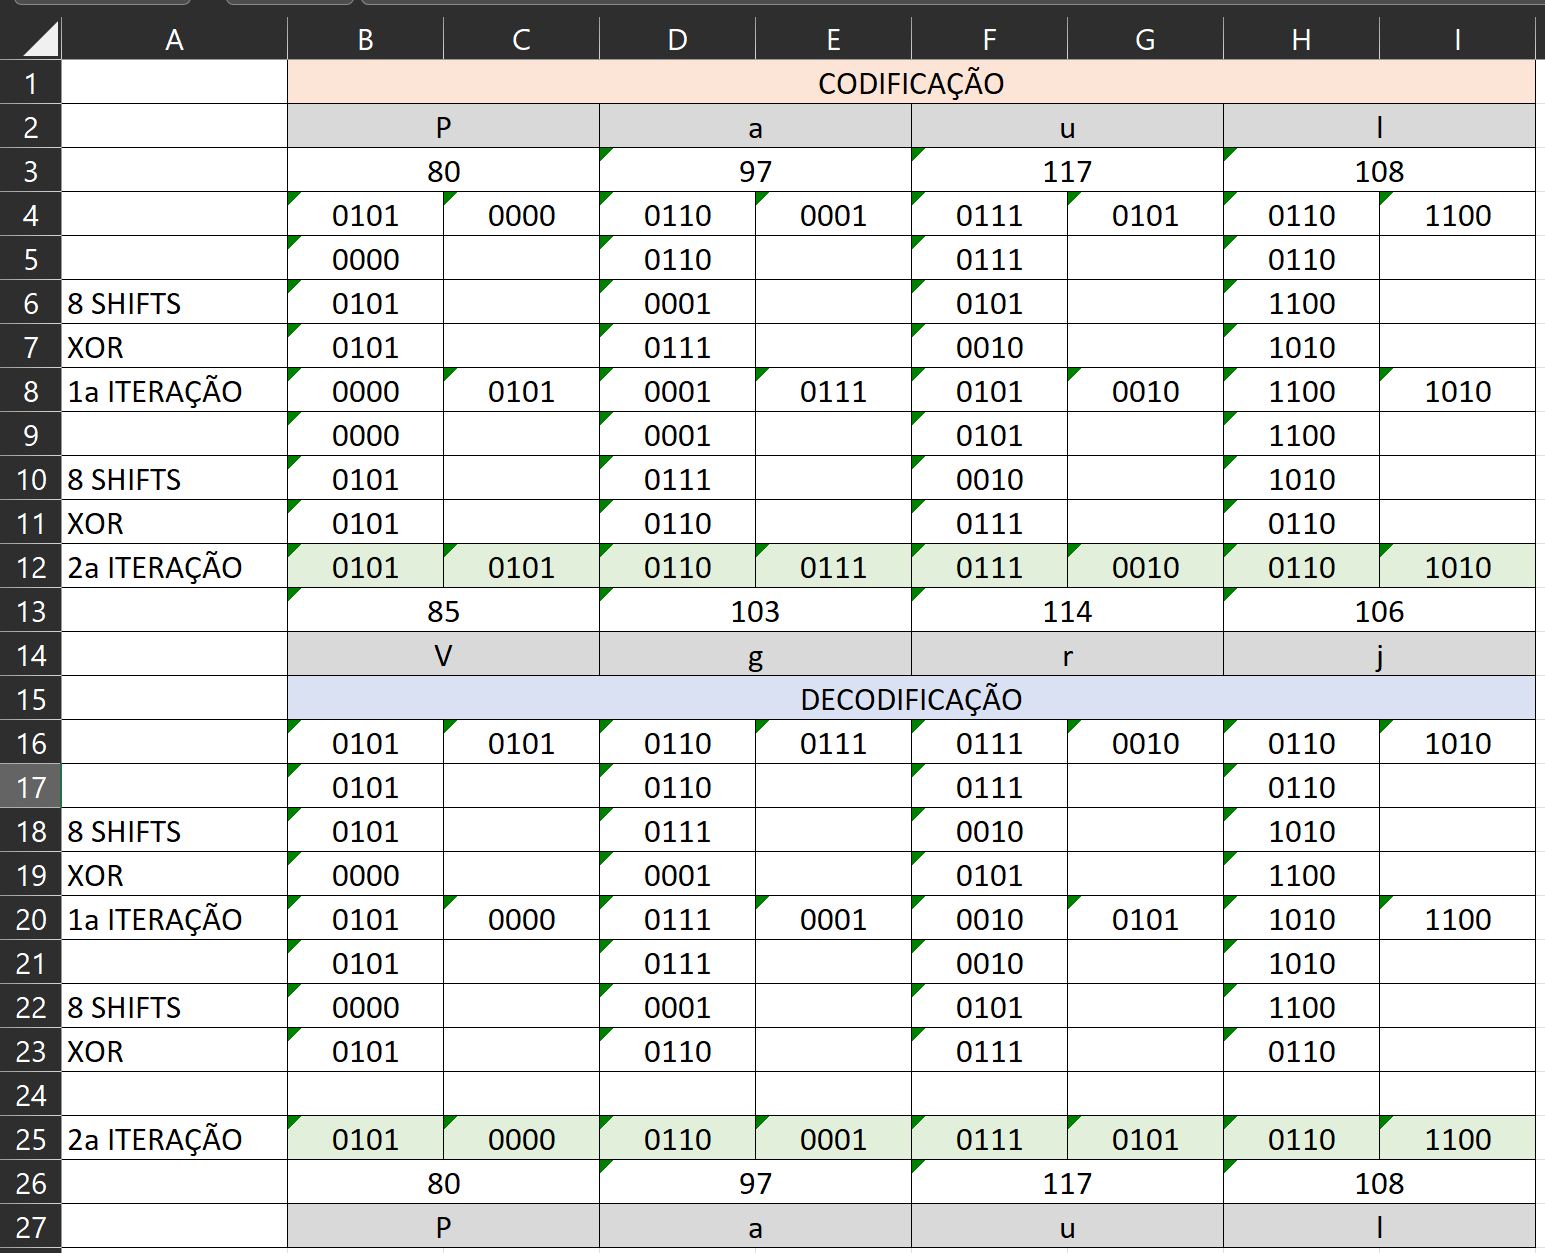
\includegraphics[width=\textwidth]{Tabela-cifra.png}
    %     \label{fig:Tabela-cifra}
    % \end{figure*}

\end{document} 